\section{Controladores \glsentryshort{sdn}}
\label{sec:sdnControllers}

Los controladores \gls{sdn}, también conocidos como sistemas operativos de red, son una pieza cable en los entornos  \gls{sdn} dado que tienen una vista global de toda la red que gestionan, que flujos atraviesan la red, estadísticas, usuarios finales, modelos y características de dichos equipos. Este controlador tiene la funcionalidad de interconectar los recursos disponibles en la red que gestiona, a aplicaciones o servicios que corran encima de él. De esta forma, cada vez que se quiera añadir una nueva funcionalidad, solo se tendrá que programar un nuevo servicio que corra encima del controlador que gestiona la red, y este a su vez se encargará de traducir las demandas del servicio a políticas de red a cada dispositivo impactado. En este matiz se puede llegar apreciar el sentido de nombre del paradigma \gls{sdn}, ya que estamos definiendo por software el comportamiento intrínseco de la red.\\
\\
% fig
\begin{figure}[ht]
    \centering
    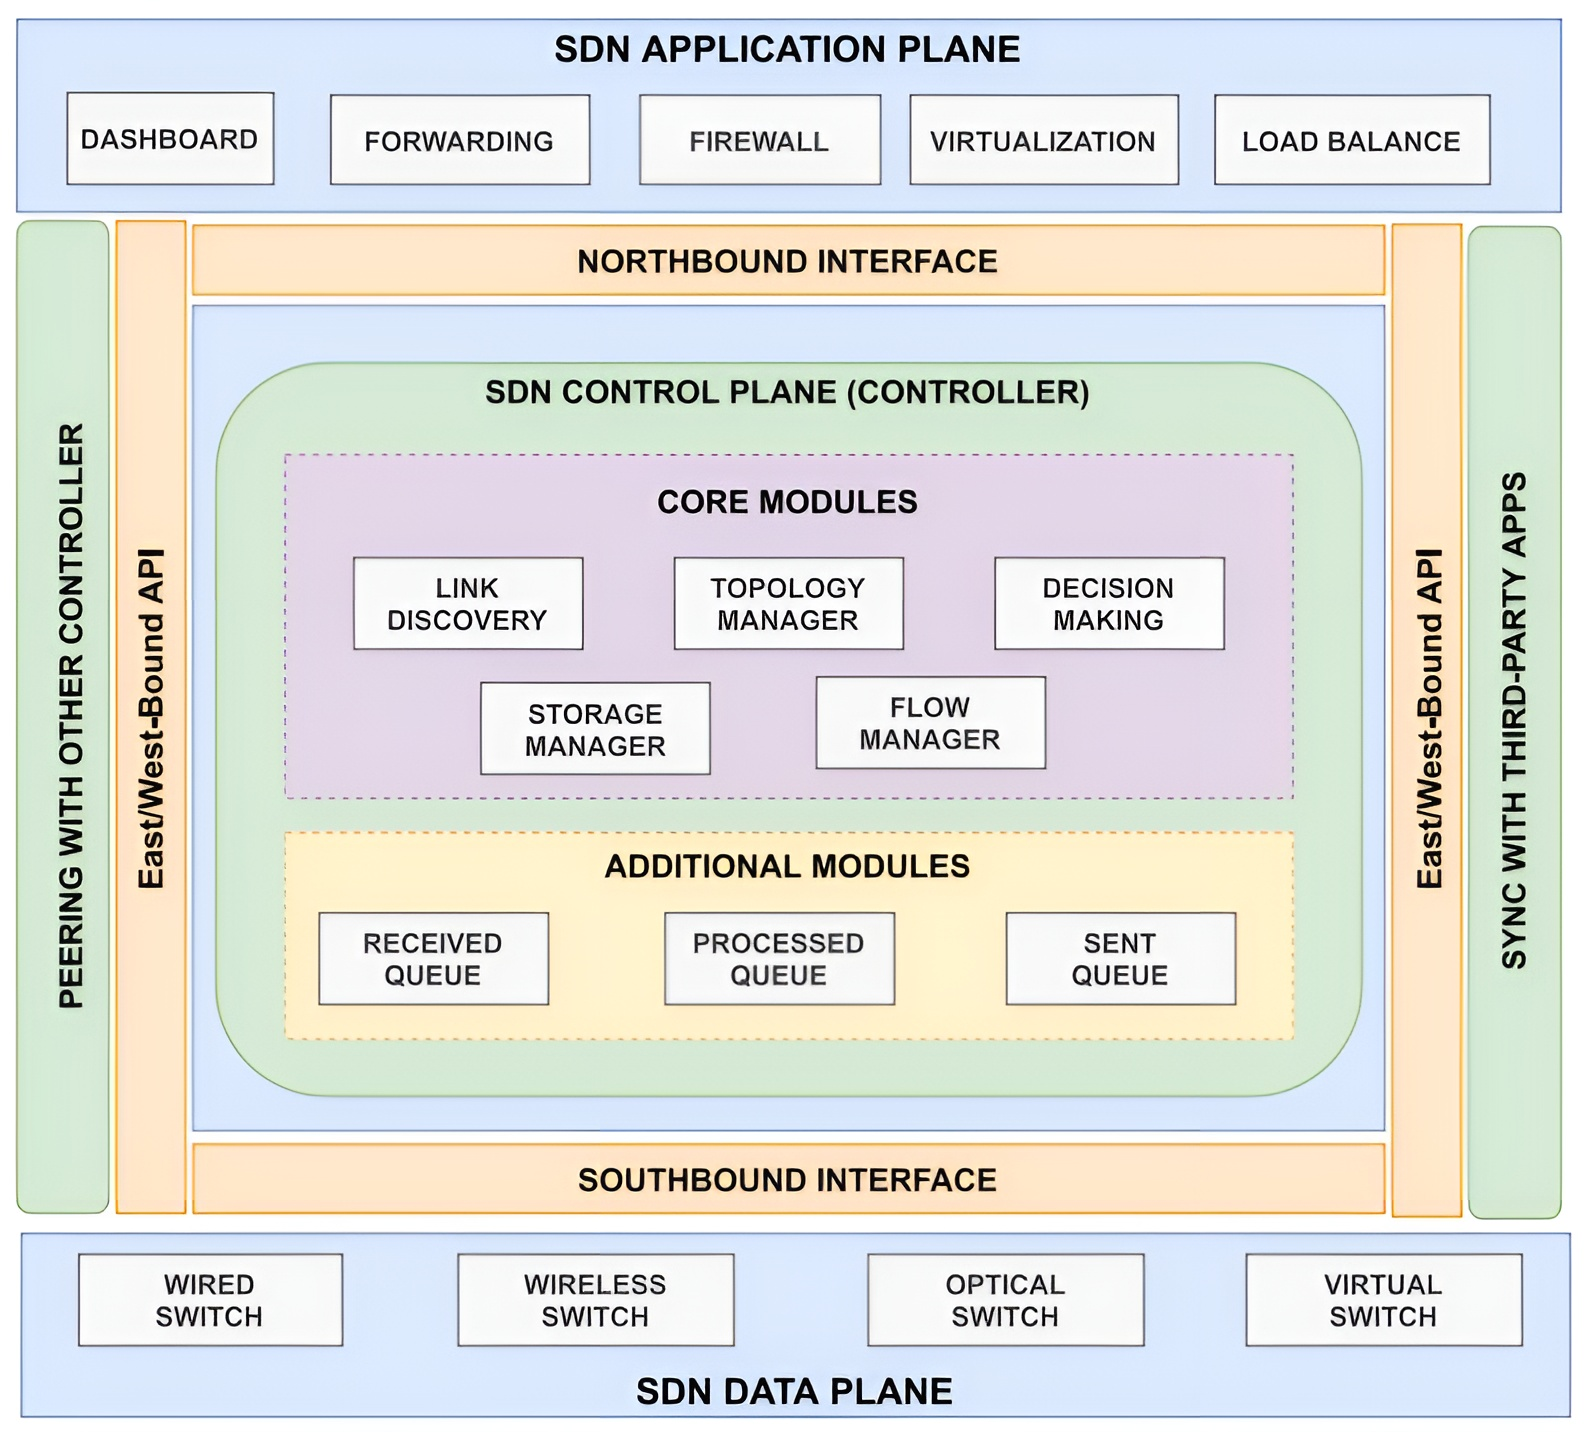
\includegraphics[width=\textwidth]{archivos/img/teoria/sdn_controllers.jpg}
    \caption{Arquitectura generica de controlador \gls{sdn} \cite{zhu2020sdn}}
    \label{fig:sdn_controllers}
\end{figure}

En la literatura hay muchas propuestas de arquitecturas para los controladores, pero en vez de ir una por una viendo las diferencias vamos a presentar la arquitectura genérica que se puede encontrar en la gran mayoría de controladores \gls{sdn}. Si nos fijamos en la figura \ref{fig:sdn_controllers}, podemos ver dos partes claramente diferenciadas, el núcleo del controlador y las interfaces del mismo. Empezando por el \textit{core}, se puede resumir que las funciones básicas del controlador están relacionadas principalmente con el descubrimiento de la topología y la gestión de los flujos de tráfico. El módulo de descubrimiento de la topología suele trabajar con el protocolo \gls{lldp}. La implementación puede variar entre controladores y aplicaciones de descubrimiento topológico, pero en términos generales, se transmite regularmente consultas utilizando mensajes \texttt{packet\_out}, los cuales viajaran por la topología física y volverán al controlador en forma de mensajes \texttt{packet\_in}, que permiten al controlador construir la topología de la red.\\
\\
Una vez que se conoce la topología de red, el controlador puede empezar a poner en marcha distintos módulos de toma de decisiones para encontrar los caminos óptimos entre los nodos de la red. Con todos los caminos ya construidos, entran en juego otros módulos del controlador como son \gls{qos} y de seguridad, los cuales pueden optar por instalar una ruta sub-óptima para satisfacer los criterios de \gls{qos} o de seguridad. De forma adicional, el controlador puede tener un recopilador de estadísticas y un gestor de colas para recopilar información sobre el rendimiento de las diferentes colas de paquetes entrantes y salientes de los dispositivos de red que gestiona, y con ellos realimentar a los módulos de \gls{qos}. Por último, tenemos uno de los módulos más importantes del controlador, el gestor de flujos. El gestor de flujos, puede variar su implementación en función de los protocolos que se utilicen en la \gls{sbi}, pero su misión es la misma, instalar reglas en los dispositivos de red que gestiona las directrices necesarias para gestionar los paquetes de un determinado flujo de una determinada manera. \\
\\
Siguiendo con otra parte fundamental del controlador \gls{sdn} genérico, son las interfaces. El controlador está rodeado de interfaces para interactuar con otras capas, superior e inferior, y otros controladores, este y oeste (E-WBIs). Empezando por la interfaz \gls{sbi}, la cual es la encargada de interconectar dispositivos \gls{sdn} con el controlador, define un conjunto de reglas, que variarán en función del protocolo que se utilice, las cuales permiten definir el procesamiento y las políticas de reenvío de los dispositivos \gls{sdn}. El protocolo OpenFlow es unas de las \gls{sbi} más utilizadas, y es un estándar de facto para la industria, con el cual podemos es definir flujos y clasificar el tráfico de red basándose en un conjunto de reglas predefinidas. Pero también se pueden encontrar otras \gls{sbi}, como por ejemplo, P4Runtime de facto el futuro para las \gls{sbi}s, o podemos encontrar algunas más \textit{legacy}, como por ejemplo, Netconf o incluso \gls{snmp}.\\
\\
Si nos vamos de la API sur, al norte, encontraremos la conocida como \gls{nbi}, la cual interconecta el controlador \gls{sdn} con las aplicaciones de los desarrolladores o los servicios que definan el comportamiento intrínseco de la red. Los controladores admiten varias interfaces de programación de aplicaciones (API) northbound, pero la mayoría de ellas se basan en la API REST. Generalmente se quiere que la interfaz \gls{nbi} sea una interfaz genérica para que limite a los desarrolladores. Para la comunicación entre controladores, se utilizan las interfaces conocidas como de este y oeste (E/WBI), las cuales no tienen una interfaz de comunicación estándar, por lo que, en función del controlador se tendrá una implementación u otra.\\
\\
A continuación, se van a ir presentando algunos de los controladores \gls{sdn} más conocidos, indicando algunas de sus virtudes y funcionamiento en particular.

\subsection{Ryu}
\label{subsec:ryu}


\subsection{ONOS}
\label{subsec:ONOS}